\documentclass[12pt,a4paper,twoside,titlepage]{article}
\usepackage{geometry}
\usepackage[]{microtype}
\usepackage[french,english]{babel}
\usepackage{enumitem}
\usepackage{setspace}
	\singlespacing
\usepackage[backend=biber]{biblatex}
\addbibresource{biblio.bib}
\usepackage[T1]{fontenc}
\usepackage{hyperref}
\usepackage{indentfirst}
\usepackage{listings}
% \usepackage[utf8]{inputenc}
\usepackage{color}
\usepackage{graphicx}
\usepackage{caption}
\usepackage{float}
\usepackage{titling}
\usepackage{pgfkeys}
\usepackage{array}
\usepackage{minted}
\usepackage[table,xcdraw]{xcolor}
\usepackage{amsmath}
\usepackage{hyperref}
\usepackage{xcolor}
\usepackage{titlesec}
\definecolor{RougeNanterre}{RGB}{227,0,27}
\usepackage[format=plain,
            font=it]{caption}
\hypersetup{
    colorlinks,
    linkcolor={black},
    citecolor={black},
    urlcolor={RougeNanterre}
}
\usepackage{fontspec}
  \setmainfont[Ligatures=TeX]{Noto Sans}
  \setsansfont[Ligatures=TeX]{Inconsolata}
  \setmonofont{Fira Mono}
% Define a new fontfamily for the subsubsection font
% Don't use \fontspec directly to change the font
\newfontfamily\subsubsectionfont[Color=RougeNanterre]{Times New Roman}
% Set formats for each heading level
\titleformat*{\section}{\Large\bfseries\sffamily\color{RougeNanterre}}
\titleformat*{\subsection}{\large\bfseries\sffamily\color{RougeNanterre}}
\titleformat*{\subsubsection}{\itshape\sffamily\color{RougeNanterre}}

\usepackage{csquotes}

\geometry{
    paper=a4paper,
    inner=3cm,
    outer=2.5cm,
    top=2.5cm,
    bottom=3.5cm
}

\usepackage{fancyhdr}
\fancyhead[RO,LE]{Ariel Nataf}
  \setlength{\headheight}{26pt}
  \renewcommand{\headrulewidth}{0.5pt}
  \renewcommand{\headrule}{\hbox to\headwidth{\color{red}\leaders\hrule height \headrulewidth\hfill}}
  \renewcommand{\footrulewidth}{0.5pt}
  \renewcommand{\footrule}{\hbox to\headwidth{\color{RougeNanterre}\leaders\hrule height \footrulewidth\hfill}}
\pagestyle{fancy}

\lstset{ %
  frame=none,
  backgroundcolor=\color{white},   % choose the background color; you must add \usepackage{color} or \usepackage{xcolor}
  basicstyle=\footnotesize\ttfamily,        % the size of the fonts that are used for the code
  breakatwhitespace=false,         % sets if automatic breaks should only happen at whitespace
  breaklines=true,                 % sets automatic line breaking
  captionpos=t,                    % sets the caption-position to bottom
  commentstyle=\color{mygreen},    % comment style
  deletekeywords={...},            % if you want to delete keywords from the given language
  escapeinside={\%*}{*)},          % if you want to add LaTeX within your code
  extendedchars=true,              % lets you use non-ASCII characters; for 8-bits encodings only, does not work with UTF-8
%  frame=single,                    % adds a frame around the code
  keepspaces=true,                 % keeps spaces in text, useful for keeping indentation of code (possibly needs columns=flexible)
  keywordstyle=\color{blue},       % keyword style
  language=,                 % the language of the code
  morekeywords={*,...},            % if you want to add more keywords to the set
  numbers=left,                    % where to put the line-numbers; possible values are (none, left, right)
  numbersep=5pt,                   % how far the line-numbers are from the code
  numberstyle=\tiny\color{mygray}, % the style that is used for the line-numbers
  rulecolor=\color{black},         % if not set, the frame-color may be changed on line-breaks within not-black text (e.g. comments (green here))
  showspaces=false,                % show spaces everywhere adding particular underscores; it overrides 'showstringspaces'
  showstringspaces=false,          % underline spaces within strings only
  showtabs=false,                  % show tabs within strings adding particular underscores
  stepnumber=1,                    % the step between two line-numbers. If it's 1, each line will be numbered
  stringstyle=\color{mymauve},     % string literal style
  tabsize=4,                       % sets default tabsize to 2 spaces
  aboveskip=3mm,
  belowskip=3mm,
}

\makeatletter
\newcommand\subTrois{\@startsection{paragraph}{4}{\z@}%
            {-2.5ex\@plus -1ex \@minus -.25ex}%
            {2.25ex \@plus .25ex}%
            {\sffamily\normalsize\itshape\color{RougeNanterre}}}
\newcommand\subQuatre{\@startsection{subparagraph}{5}{\z@}%
            {-2.5ex\@plus -1ex \@minus -.25ex}%
            {2.25ex \@plus .25ex}%
            {\sffamily\normalsize\itshape\color{RougeNanterre}}}
\newcommand\subCinq{\@startsection{subparagraph}{6}{\z@}%
            {-2.5ex\@plus -1ex \@minus -.25ex}%
            {2.25ex \@plus .25ex}%
            {\sffamily\normalsize\itshape\color{RougeNanterre}}}        
\makeatother

\newcommand{\coverpage}[1]{%
\begin{titlepage}
\newcommand{\HRule}{\rule{\linewidth}{0.5mm}} % Defines a new command for the horizontal lines, change thickness here

\center % Center everything on the page
 
%----------------------------------------------------------------------------------------
%	HEADING SECTIONS
%----------------------------------------------------------------------------------------

\textsc{\LARGE Rapport de stage de fin d'année}\\[0.3cm] % Name of your university/college
\textsc{\LARGE 1ère année de Master  }\\[0.3cm]
\textsc{\Large \color{RougeNanterre} Université Paris Nanterre }\\[0.3cm]
\textsc{\LARGE  à \color{RougeNanterre} GFI Informatique}\\[0.5cm] % Major heading such as course name
 % Minor heading such as course title

%--------------------------------------------------------------------------------
%	TITLE SECTION
%--------------------------------------------------------------------------------

\HRule \\[0.4cm]
{\sffamily \huge \bfseries Étude de caméras}\\[0.2cm]
{\sffamily \huge \bfseries et d'algorithmes de tracking}\\[0.1cm]
{\sffamily \huge \bfseries pour la Computer Vision sur OpenCV}\\[0.3cm]
% Title of your document
\HRule \\[1.5cm]

\vspace*{\fill}

%--------------------------------------------------------------------------------
%	AUTHOR SECTION
%--------------------------------------------------------------------------------

\begin{minipage}{0.4\textwidth}
\begin{flushleft} \large
Étudiant~:\\
\color{RougeNanterre}Ariel NATAF% Your name
\end{flushleft}
\end{minipage}
~
\begin{minipage}{0.4\textwidth}
\begin{flushright} \large
Maître de stage~:\\
\color{RougeNanterre}Jean-Paul MULLER% Supervisor's Name
\end{flushright}
\end{minipage}\\[1cm]

% If you don't want a supervisor, uncomment the two lines below and remove the section above
%\Large \emph{Author:}\\
%John \textsc{Smith}\\[3cm] % Your name

%--------------------------------------------------------------------------------
%	LOGO SECTION
%--------------------------------------------------------------------------------


\includegraphics{img/Logo_GFI_2011.jpg}\\[1cm]

\includegraphics{img/logo_Nanterre.jpg}\\[1cm]% Include a department/university logo - this will require the graphicx package

%--------------------------------------------------------------------------------
%	DATE SECTION
%--------------------------------------------------------------------------------

{\large avril-juillet \color{RougeNanterre}2018}\\[1cm] % Date, change the \today to a set date if you want to be precise
 
%--------------------------------------------------------------------------------

\vfill % Fill the rest of the page with whitespace
\end{titlepage}
}

% Custom arguments for /fig command
\pgfkeys{
 /fig/.is family, /fig,
 default/.style = 
  {scale = 1,
   angle = 0},
 scale/.estore in = \figScale,
 angle/.estore in = \figAngle
}
\newcommand{\fig}[2][]{%
	\pgfkeys{/fig, default, #1}%
	\begin{figure}[H]%
    \centering
    \includegraphics[angle=\figAngle,width=\figScale\textwidth]{#2}%
	\end{figure}%
}

\newcommand{\filename}[1]{%
	\texttt{#1}%
}

\newcommand{\vhdl}[1]{%
  \lstinputlisting[language=vhdl]{#1}
}

\newcommand*\paths[1]{\lstset{inputpath=#1}\graphicspath{#1}}



\setcounter{secnumdepth}{7} % how many sectioning levels to assign numbers to
\setcounter{tocdepth}{7}    % how many sectioning levels to show in ToC

\title{Stage GFI 2018\\ }
\author{Ariel NATAF}
\date{LING/TRST 415: Spring 2017}
\begin{document}
\selectlanguage{french}
 \coverpage{assessment}
\vspace*{\fill}
\cleardoublepage
	\tableofcontents
\setlength{\parskip}{\baselineskip}%
\vspace*{\fill}
\newpage
\cleardoublepage
\section*{Introduction}

% Introduction : C’est un vrai résumé de l’ensemble du mémoire : contexte, problématique, aperçu (i.e. indication rapide) de votre contribution et son originalité, plan du reste du mémoire.

Le stage a eu lieu au sein de l'entreprise GFI dans le service de la "Forge" au \textbf{157 Boulevard Macdonald à Paris}. Il s'est déroulé \textbf{du 9 avril au 31 juillet 2018}.

Un projet de Computer Vision a été mis en place au sein de la forge pour répondre à la demande d'un client (une commune) qui souhaitait être capable d'\textbf{analyser la circulation à l'aide de caméra de surveillances}.

Au sein de la forge, le besoin de tester des caméras et de comparer des algorithmes s'est exprimé. J'ai consacré les premiers mois de mon stage à chercher à apporter des réponses à ces problèmes. 

Le rapport présentera d’abord l'entreprise et le service dans lequel j'ai travaillé, puis va tourner autour des problèmes rencontrés et des solutions présentées avant de conclure avec un bilan.

\section{GFI}

GFI est une ESN et le stage a eu lieu dans les locaux de la \textbf{Forge}.
\subsection{L'entreprise}

Fondée en 1995, GFI est une Entreprise de Service Numérique (\textit{ESN}) dont le siège se trouve à Saint-Ouen en France. Elle compte aujourd'hui 16 000 collaborateurs dans une vingtaine de pays (Suisse, Belgique, Espagne, Brésil...). Son chiffre d'affaires s'élève à 1 132 M€ en 2017 et 74,5 \% de son activité se situe en France.
\begin{quotation}
\textit{Notre stratégie~: Être reconnu comme le 1er acteur régional des services et solutions à valeur ajoutée.
}
Vincent Rouaix - Président-Directeur Général
\end{quotation}
Pour parvenir à cela GFI a trois leviers de croissances~: 
\begin{itemize}
\item La \textbf{proximité}, avec des implantations régionales qui ont vocation à être souple et réactives pour être à proximité des clients.
\item L'\textbf{industrialisation}, avec à la clef des gains de productivité, une réduction du\textit{ time-to-market} et des coûts optimisés.
\item L'\textbf{innovation} pour apporter des solutions innovantes.
\end{itemize}

Afin de concrétiser le levier de l'innovation, GFI a notamment lancé un \textit{Fablab} dans les locaux du \textbf{Cargo} dans les 19e arrondissement de Paris.

\subsection{La Forge}

\begin{minipage}{0.3\textwidth}
  \centering
  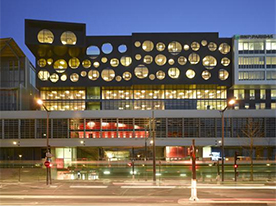
\includegraphics[width=5cm, trim={0 0.5cm 0 0.2cm},clip]{img/cargo.jpg}
\end{minipage}
\hfill%
\begin{minipage}[adjusting]{0.6\textwidth}
 \hspace{\parindent}En octobre 2016, GFI a lancé son Fablab dans les locaux de l'incubateur \textit{Le Cargo} à Paris. Ce Fablab vient renforcer la phase amont du processus d’\textbf{idea generation}. Au travers d’ateliers thématiques, il a vocation de prototyper les cas d’usage des clients.  Pour prolonger cette initiative, GFI a lancé \textit{La Forge}.
\end{minipage}\par

La Forge a pour vocation d'accompagner les entreprises dans l'industrialisation du prototype. Ses experts conseillent les entreprises en matière de financement, de sourcing matériel ou encore de maintenance de l'innovation. En amont, ils ont aussi un rôle de veille technologique et organisent des journées d'acculturation aux «~\textit{buzzwords}~» (machine learning, chatbot...)~: ce que ces nouvelles techniques permettent ou ne permettent pas, en donnant les clefs de compréhensions aux clients pour qu'ils se projettent...

\subsection{Organisation}

La Forge gère plusieurs \textbf{missions en parallèle}, elles peuvent concerner la \textit{Computer Vision}, mais aussi des \textit{chatbots}, des questions de \textit{blockchain}. L'équipe au complet compte près d'une vingtaine de personne qui se répartissent ces différentes missions.

L'équipe est \textbf{composée} d'employés de GFI à plein temps, d'alternants et de stagiaires. 

% AGILE ?


\newpage

\newpage
\section*{Missions pour contribuer aux travaux de \textit{Computer Vision}}

Les missions que j'ai reçu à l'occasion de mon stage ont eu pour objectif d'aider à identifier différents éléments afin d'aider à choisir parmi ces éléments ceux qui sont les plus adaptés au besoin dans le futur. Ainsi dans le cadre de la computer Vision ceci s'est concrétisé comme~:
\begin{enumerate}
\item Le test de \textbf{connexion} de caméra,
\item Une réflexion sur comment tester leur \textbf{connexion}.
\item L'utilisation  d'une librairie de \textit{Computer Vision}, \textbf{OpenCV et à en comparer différentes fonctions}.
\end{enumerate}
\cleardoublepage
\section{Connexion des caméras IP}

	L'objectif de cette mission a été d'étudier différentes caméras IP misent à ma disposition, quels sont leurs fonctionnalités, et établir un rapport qui servira à guider l'achat de nouvelles caméras.
    
    Pour cette mission, la réflexion tournera d'abord autour de l'\textbf{état de l'art}, puis sur les \textbf{difficultés rencontrées} et enfin sur des \textbf{améliorations possibles} à l'étude de connexion des caméras IP.

  \subsection{État de l'art}
  
  L’état de l'art se décompose ici en l'étude des \textbf{caméras IP} et des \textbf{solutions existantes} pour la connexion de ces caméras
 	 \subsubsection{Les caméras IP}
        Une \textit{caméra IP}, est une \textbf{caméra numérique} généralement utilisée pour la \textbf{surveillance}. Contrairement à des caméras dites CCTV (\textit{Closed-circuit television}), la caméra IP peut envoyer et recevoir des données via un \textbf{réseau informatique et internet}. Bien que la plupart des caméras pouvant faire cela sont des webcams, le terme \textit{caméra IP} est généralement utilisée 
dans le cadre de la surveillance qui peut être directement accédé par une connexion réseau.
        
        Une caméra IP peut être câblée avec du \textit{RJ45} vers un \textit{routeur} ou «~box ADSL~», ce qui lui permet à la fois d'être alimentée et les images visionnées sur le réseau, ou alors par Wi-Fi (une alimentation en courant électrique devient alors nécessaire). \textbf{Contrairement aux Webcams}, la compatibilité avec les logiciels de visioconférence n'est pas toujours garantie.
        
 	 \subsubsection{Solutions existantes}
     
     La connexion aux caméras IP n'est pas un monde vierge de toute fondation, on y trouve des \textbf{interfaces}, des \textbf{flux \textit{RSTP}}, et une \textbf{norme \textit{Onvif}}
     
		\subTrois{Les interfaces constructeurs}
        Les caméras IP sont en règle générale accompagnées dans leur partie logicielle d'une interface utilisateur. Ces interfaces permettent de configurer les caméras et éventuellement d'accéder au flux vidéo. L'approche de conception de ces interfaces varie grandement en fonction du public visé et de l'utilisation préconisée.

Voici quelques exemples d'interface rencontrée au cours du stage :
\begin{itemize}
\item         \textbf{D-Link}, une interface complète, localisée en français, conçue pour être facilement configurable par des professionnels et des amateurs, bien qu'elle nécessite la connaissance de son adresse IP pour y accéder.
\item         \textbf{XIAOMI, Xiao Fang (Fang Hacks)}, XIAOMI n'étant pas encore implanté en France quand il a fallu essayer ce modèle (avant le 22 mai 2018~\cite{Xiaomi}), son service de Cloud n'était \textit{a fortiori} pas non plus accessible sur le territoire français. Il a fallu installer nouveau système d'exploitation sur la caméra, le \textit{«~Fang Hacks~»}~\cite{FangHacks}. Cette interface est très rudimentaire et ne contient qu'une interface destinée à gérer la connexion. Elle s'adresse surtout à un  public de technophiles ayant envie d'utiliser cette caméra premier prix.
\item         \textbf{VR CAM}, marque d'origine chinoise, cible un très grand public et permet de connecter et d'utiliser leurs caméras via leur application mobile~\cite{VRCam}. Une utilisation via une autre médium n'est pas prévue par le constructeur. L'interface de l'application a visiblement été localisée en utilisant un traducteur automatique à partir du chinois.
\end{itemize}


\begin{minipage}{0.3265\textwidth}
\begin{figure}[H]
	\centering
	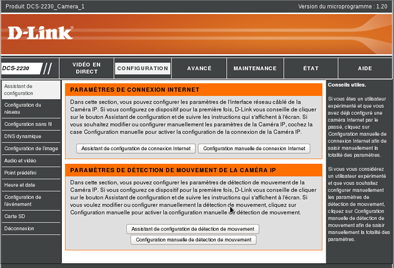
\includegraphics[width=4.5cm]{img/d-link_web.png}
    \caption{\\D-Link}
\end{figure}
\end{minipage}
\begin{minipage}{0.3265\textwidth}
\begin{figure}[H]
	\centering
	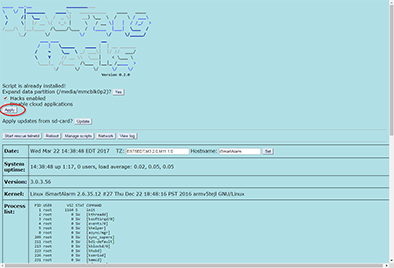
\includegraphics[width=4.5cm]{img/fanghacks.png}
    \caption{\\Fang Hacks}
\end{figure}
\end{minipage}
\begin{minipage}{0.3265\textwidth}
\begin{figure}[H]
	\centering
	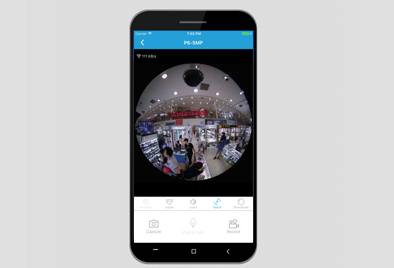
\includegraphics[width=4.5cm]{img/vrcam_mob.png}
    \caption{\\VRCAM}
\end{figure}
\end{minipage}
        
		\subTrois{Le RTSP}
\textit{RTSP} ou \textit{Real Time Streaming Protocol} (protocole de streaming temps-réel) est un protocole de communication de niveau applicatif(niveau 7 du modèle \textit{OSI}) destiné aux systèmes de streaming média. Il permet de \textbf{contrôler un serveur de média} à distance, offrant des fonctionnalités typiques d'un lecteur vidéo telles que «~lecture~» et «~pause~», et permettant un accès en fonction de la position temporelle.~\cite{RTSPwiki}

La \textbf{transmission des données} de streaming elle-même n'est pas la tâche du protocole \textit{RTSP}. La plupart des servers \textit{RTSP} utilise le \textit{RTP} (\textit{Real-time Transport Protocol}) en conjonction avec \textit{RTCP} (\textit{with Real-time Control Protocol}) pour la distribution du stream média.~\cite{RTSP}

Le \textit{RTSP} permet le \textbf{multicast} pour la diffusion simultanée à plusieurs clients. Une variété de formats vidéos et audio sont supportés tel que .\textit{264}, \textit{MPEG4}, \textit{MJPEG}, \textit{AAC}, \textit{WMV} etc.

Son utilisation peut se faire avec le logiciel de lecture vidéo \textit{VLC}, ou par un programme qui utilise la librairie \textbf{OpenCV} par exemple.

		\subTrois{La norme \textit{Onvif}}
        
          \begin{minipage}{0.2\textwidth}
  \centering
  
\includegraphics[width=4cm]{img/logoonvif.png}
\end{minipage}
\hfill%
\begin{minipage}{0.7\textwidth}
Le protocole \textit{ONVIF}~\cite{Onvif} est l'acronyme du \textbf{O}pen \textbf{N}etwork \textbf{V}ideo \textbf{I}nterface \textbf{F}orum. Le principe remonte au début des années 2010, où les grandes marques du domaine telles que \textit{Sony} ou \textit{Bosch} ont proposé de mettre en place un forum industriel qui vise à développer une \textbf{norme mondiale d'inter-opérabilité} des produits de sécurité IP. 
  \end{minipage}\par
  
  \textit{ONVIF} travaille aussi avec des groupes de standardisation tel qu'\textit{IEC} (\textit{International Electrotechnical Commission}), \textit{CENELEC} et \textit{ISO} pour leur faire adopter les spécifications ONVIF. Ces spécifications sont des services web, utilisent des standards ouverts dont \textit{XML}, \textit{SOAP} et \textit{WSDL} pour définir la communication entre deux appareils électroniques dans un réseau IP.

Ceci permet aux produits de vidéo-surveillance IP \textbf{de pouvoir échanger des informations} entre eux, même s'ils proviennent \textbf{de différent fabricants}. Cependant il appartient à ces fabricants d'implémenter ce standard dans leurs produits. Toutes les caméras Onvif n'auront pas la même liste exhaustive de contrôles, ni la même qualité d'implémentation.

La connexion via le protocole Onvif peut se faire en passant par le logiciel open source \textit{ONVIF Device Manager}~\cite{Onvifdm}. Pour la connexion, il suffit de renseigner l’adresse \textbf{[IP]:[Port Onvif]} de la caméra concernée en utilisant l'interface du logiciel.

\begin{figure}[H]
	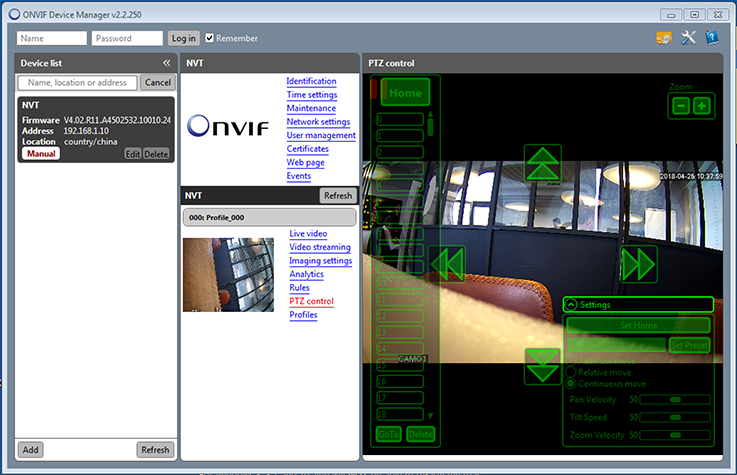
\includegraphics[width=0.7\textwidth]{img/onvifecran.png}
    \centering
    \caption{Interface d'\textit{ONVIF Device Manager}}
\end{figure}

Durant cette mission, des difficultés ont été rencontrées.

	\subsection{Difficultés rencontrées}

Les caméras qui m'ont été demandées d'étudier ne venaient pas toujours avec toutes les clefs. Cela s'illustre par :
\begin{enumerate}
\itemsep -0.5em 
\item la documentation parfois lacunaire,
\item des soucis pour les connecter au réseau,
\item une compatibilité logicielle,
\item des formats de flux vidéo.
\end{enumerate}


		\subsubsection{La documentation}
Lors de ma mission, certaines caméras à connecter n'avaient pas forcément une documentation très fournie.

Par exemple une caméra (\textit{Escam Q1039}) avait comme  documentation officielle une vidéo sur youtube en russe.

\begin{figure}[H]
	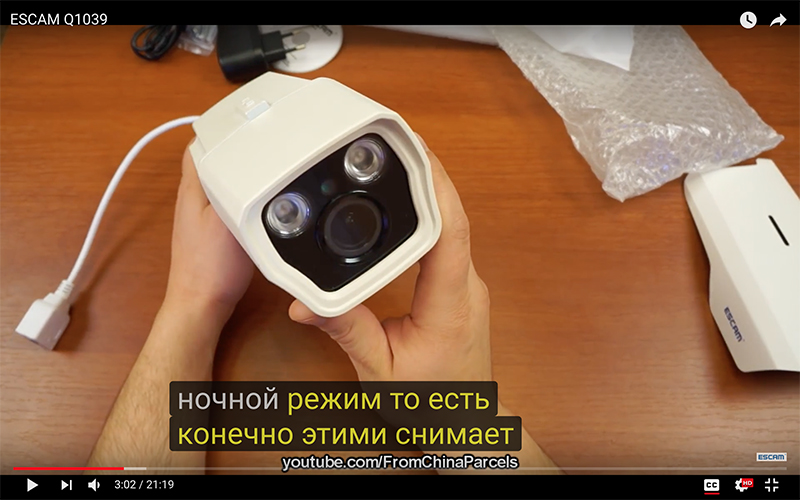
\includegraphics[width=0.8\textwidth]{img/escam_russe.jpg}
    \centering
    \caption{vidéo explicative en russe\\publiée sur la chaîne Youtube d’EScam~\cite{EscamVid}}
    \end{figure}
    Le manque de documentation peut s'avérer problématique. En effet, chaque fabricant dans l'installation de la partie logiciel de la caméra attribut notamment des adresses pour accéder aux flux vidéos pour \textbf{RTSP} ou \textbf{Onvif} par exemple.
    
    Toutefois, il reste possible de parfois retrouver certaines de ces informations. Par exemple le site \textit{ipsyConnect} met à disposition une liste de caméra avec des adresses pour se connecter en \textit{RTSP}.~\cite{ispy}
\begin{figure}[H]
    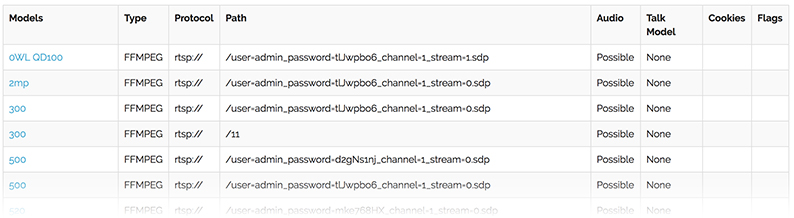
\includegraphics{img/liste_ispy.jpg}
    \centering
    \caption{extrait de la liste de caméra EScam sur ISpyConnect}
\end{figure}

		\subsubsection{La connexion au réseau}
    Pour configurer une caméra IP une connexion au routeur internet est nécessaire.
        
	L'installation des locaux de la «~\textit{Forge}~» est faite de telle façon à ce qu'internet soit accessible par wi-fi uniquement. L'accès au routeur n'est pas possible. La connexion a donc dû se faire sans passer par le réseau internet. Pour établir une connexion, la connexion s'est établie en pair à pair avec deux nœuds en branchant directement un câble \textit{RJ45} à l'ordinateur et à la caméra IP.
    
    Cette configuration réseaux particulière a permis d'explorer les fonctionnalités des caméras, mais sans avoir accès un internet ce qui a pu poser problème lors de la recherche d'informations au cours de l'utilisation.
    
		\subsubsection{La compatibilité logicielle}
	Durant le stage j'utilise mon ordinateur personnel. Un Macbook Pro avec \textbf{MacOS}. Cependant certains logiciels ne sont pas compatible avec ce système d'exploitation. Un appareil a même son interface web qui utilise \textbf{ActiveX}. ActiveX n'est compatible qu'avec \textbf{Internet Explorer} qui n'est pas compatible avec MacOs. 
    
    Pour contourner ce problème j'ai dû installer une \textbf{Machine Virtuelle Windows} pour lancer Internet Explorer et y utiliser Active X.
\begin{figure}[H]
    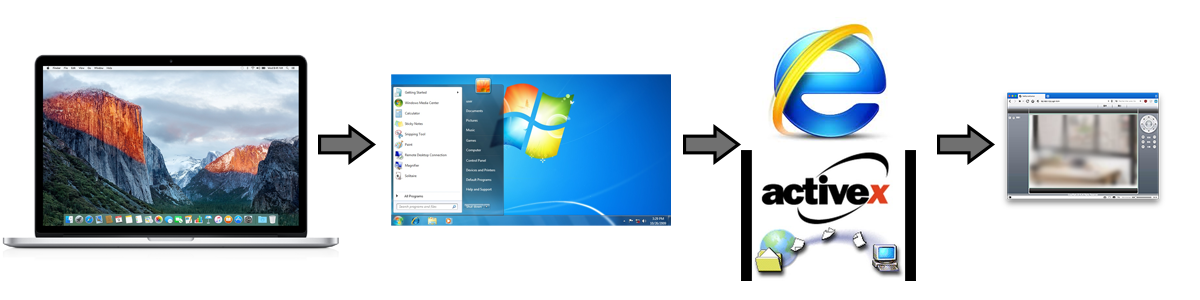
\includegraphics[width=0.8\textwidth]{img/Aesthetic_graph.png}
    \centering
    \caption{Environnement de travail ad hoc}
\end{figure}

    \subsubsection{Le format de flux vidéo}
    Chaque fabricant ayant le droit de faire comme bon lui semble, certaines caméras peuvent avoir des formats de flux vidéos qui ne sont pas exploitables. En effet, il est arrivé qu'une caméra ne retourne pas un flux vidéo, mais une image au format \textit{.jpeg} en se connectant avec l'adresse \textbf{RTSP}. Cette méthode a réputation d'avoir des images de meilleures qualité au prix d'une vidéo plus saccadée. Avec une vidéo mois fluide, l'étude du déplacement d'un objet est plus compliquée.

Il a été décidé d'écarter les caméras qui renvoient un flux d'image qui n'est pas au format vidéo. 

Des \textbf{améliorations sont possibles}. 

\subsection{Améliorations possibles}

  L'étude des caméras c'est fait à partir d'un nombre réduit de caméras (quatre). Pousser l'étude consisterai à \textbf{augmenter le nombre de caméras}. Ainsi de nouveaux problèmes vont se dévoiler et alors de nouveaux critères vont émerger pour \textbf{affiner le guide pour l'achat de caméras}.

  Un autre aspect serait de pouvoir \textbf{connecter les caméras à un router et y accéder à distance}. En raison des limitations techniques cet aspect à été mis entre parenthèse, mais il reste néanmoins un aspect fondamental des caméras IP.

% ------------------------------------------------
% /\/\/\/\/\/\/\/\/\/\/\/\/\/\/\/\/\/\/\/\/\/\/\/\
% ------------------------------------------------
\cleardoublepage
\section{Établissement d'un protocole de test de caméras}
La deuxième partie de ma mission d'étude de caméra est d'effectuer un travail de veille. Il sert à établir un protocole de test de ces caméras. Ces tests ont pour vocation d'estimer la qualité des enregistrements vidéos et d'en reconnaître les plus adaptés au besoin de la \textit{Computer Vision}.  

La présentation de cette mission commence par un \textbf{état de l'art}, suivie d'une de ma \textbf{contribution} qui sera ensuite \textbf{évaluer} et des \textbf{perspectives} possibles.

  \subsection{État de l'art}
    Les tests de qualité des caméras est essentiellement basée sur l'évaluation de la netteté de l'image. Les sociétés qui effectuent les tests de caméras ont leurs propres méthodologies, mais ont tendance à s'inspirer de la \textbf{norme ISO-12233}~\cite{ISO12233}. Cette norme présente notamment un panneau qui sert à évaluer la netteté de l'image. Cette norme est mise à jour environ tout les quatre ans. La dernière version en date est celle de 2017.

  \begin{minipage}{0.45\textwidth}
  \begin{figure}[H]
      \centering
      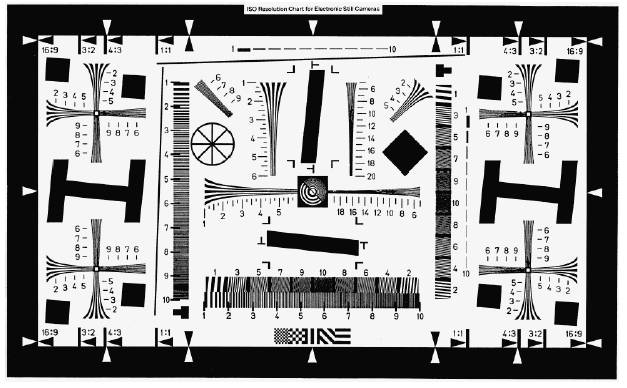
\includegraphics[width=6cm]{img/ISO12233-2000.jpg}
      \caption{ISO12233-2000}
  \end{figure}
  \end{minipage}
  \begin{minipage}{0.5\textwidth}
  \begin{figure}[H]
      \centering
      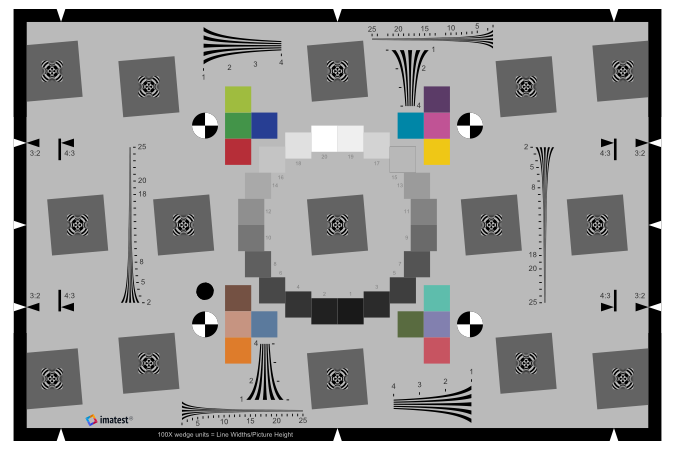
\includegraphics[width=6cm]{img/ISO12233-2017.png}
      \caption{ISO12233-2017}
  \end{figure}
  \end{minipage}

    La netteté est analysée à partir de zébrures de plus en plus resserrées, plus l'image sera nette, plus chacune de ses rayures seront distinctes. L'analyse se fait avec des algorithmes dit de \textbf{MTF} (pour \textbf{M}odulation \textbf{T}ransfer \textbf{F}unction)~\cite{MTF}. Plusieurs programmes payants permettent ces analyses (\textit{IMATEST}, \textit{QuickMTF}), il est également possible d'utiliser un script python avec des librairies gratuites. Les résultats obtenus vont toutefois varier en fonction de l'implémentation de l'algorithme.

    \begin{figure}[H]
      \centering
      
\includegraphics[width=0.8\textwidth]{img/mtf.png}
      \caption{Effet de perte de netteté sur les zébrures}
  \end{figure}

  Les panneaux de la norme \textbf{ISO-12233} disposent des rayures de façon à prendre en compte les courbures de la lentille de l'appareil. L'image ayant tendance à être plus nette au centre que sur les bords.
  
  Pour avoir une meilleure luminosité de la façon la plus consistante possible, les images sont prises en intérieur, avec des lumières neutres et en utilisant des panneaux servant filtrer la lumière pour la rendre plus diffuse et éviter les reflets.
  
  La capacité d'une caméra à produire une image nette varie en fonction de plusieurs facteurs comme la \textbf{luminosité}, la \textbf{distance focale} ou le \textbf{mouvement}. 
  
  \subsection{Contributions}
  La finalité de cette mission a été de \textbf{présenter un document} qui compile les conclusions du \textbf{travail de veille} pour les caméras. Ce document a pris la forme d'une présentation \textit{Microsoft Power Point}.
  
  Une solution naïve pour les tests de caméra dans un environnement \textbf{contrôlable et prédicable} est de filmer un écran qui diffuse une vidéo. Cette solution permet en théorie de contrôler simplement toutes les variables comme la luminosité, les éléments de l'image, le mouvement. Une solution idéale en théorie, en pratique elle présente plusieurs \textbf{inconvénients}.
  
  Filmer un écran qui diffuse une vidéo ne revient pas au même que de filmer directement la vidéo. L'écran est plat, projette de la lumière et en reflète. Ceci a pour effet de dégrader fortement la qualité de l'image. En conséquence l'image que filme la caméra n'est plus de qualité suffisante pour tester la qualité de l'image en situation réelle.
  
	\begin{figure}[H]
      \centering
      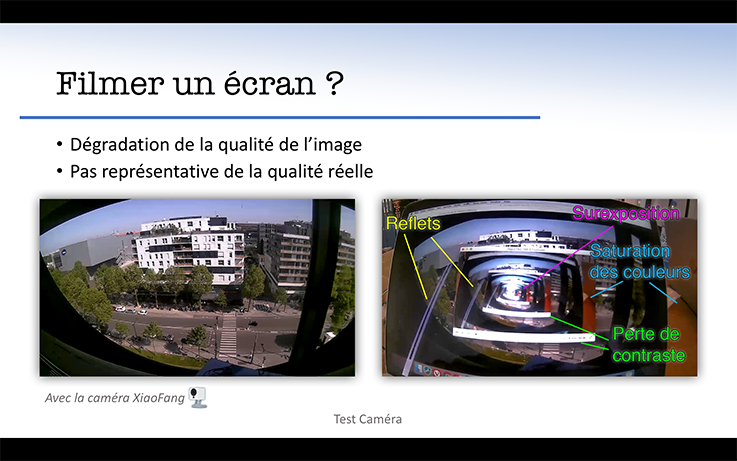
\includegraphics[width=12cm]{img/CamTestEcran.png}
      \caption{Écarter explicitement cette solution\\et pourquoi}
	\end{figure}
  
  La solution retenue utilise donc un support \textbf{analogique} pour une meilleure fidélité d'image.
  
  L'installation voulue serait une installation qui correspond à l'état de l'art (lumière neutre, panneau diffuseur de lumière, trépied pour la caméra) et sans un logiciel particulier pour évaluer la netteté. La luminosité ayant un effet important sur la qualité d'image, l'utilisation d'un \textbf{photomètre}, appareil servant à mesurer les niveaux de luminosité, est recommandé pour s'assurer des bonnes conditions de tests.
  
  Les tests principaux se font en utilisant un \textbf{panneau ISO-12233} compatible.
  
\begin{minipage}{0.4\textwidth}
  \begin{figure}[H]
    \centering
    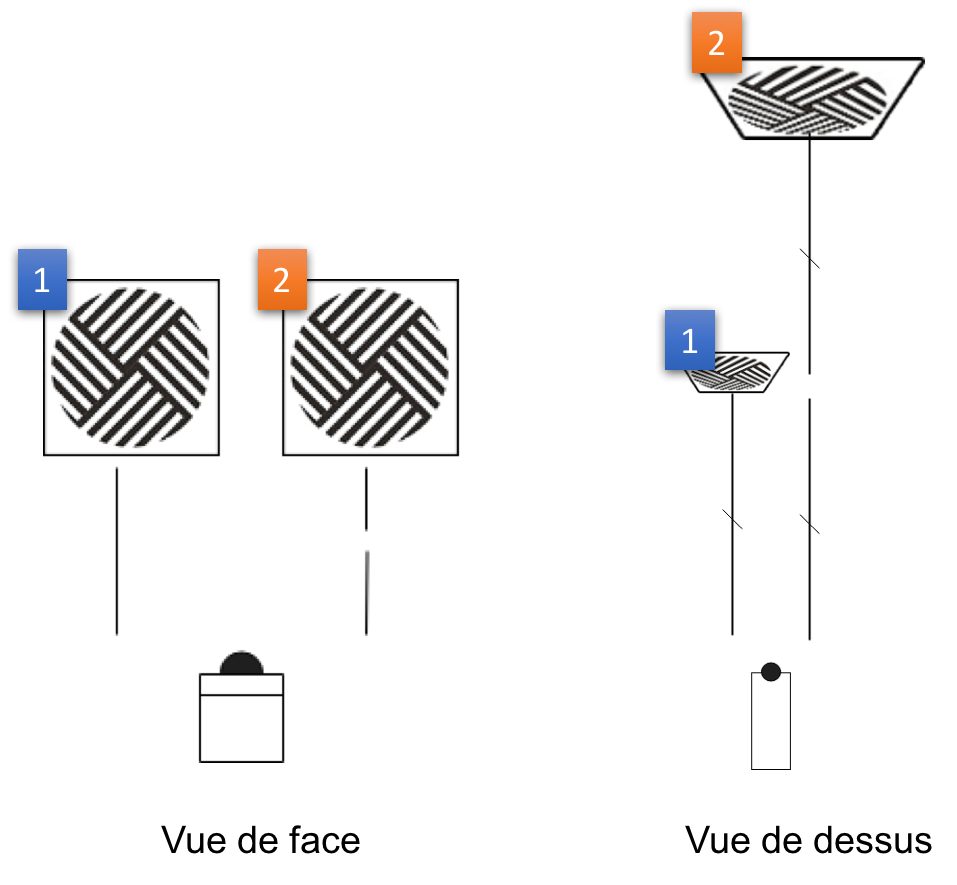
\includegraphics[width=\textwidth]{img/test_focal.png}
    \caption{schéma pour l'installation des tests de focal}
  \end{figure}
\end{minipage}
\hfill%
\begin{minipage}[adjusting]{0.52\textwidth}
  Les vidéos devant tenir compte de la \textbf{profondeur de champ}, il est intéressant de chercher à s'assurer que les caméras retenues puissent offrir une bonne qualité d'image à différent niveau de profondeur.
L'idée pour ce test est de prendre deux panneaux, de tailles différentes placés à une distance calculée telle que les deux panneaux apparaissent de même taille. On analyse la netteté de l'image avec les deux panneaux. \textbf{Si la caméra est capable de bien gérer bien les profondeurs d'image, les deux panneaux seront nets}. Sinon, un panneau sera plus flou que l'autre. 
\end{minipage}\par

Pour l'analyse de la \textbf{qualité d'image lors du mouvement}, un autocollant posé sur un démonstrateur capable de le déplacer selon un trajet défini. On analyse la netteté de l'image lors du déplacement sur plusieurs directions.


\begin{minipage}{0.2\textwidth}
\begin{figure}[H]
    
\includegraphics[width=0.5\textwidth]{img/grille_couleur.png}
    \centering
    \caption{exemple de grille de couleur}
\end{figure}
\end{minipage}
\hfill%
\begin{minipage}[adjusting]{0.7\textwidth}
Un autre critère qui n'est pas lié à la netteté de l'image est la \textbf{fidélité des couleurs}. Certains algorithmes de Computer Vision passent par une sélection de couleur. Pour tester la fidélité, on capture l'image d'un panneau avec une grille de couleurs avec des valeurs cibles connues. 
\end{minipage}\par

\subsection{Évaluation et perspectives}

La démarche de protocole de test ne \textbf{s'est jamais concrétisée}. Les moyens à mettre en place n'étaient pas justifiés par le besoin estimé de réaliser ces tests. Sans réaliser ces tests il est \textbf{difficile d'estimer la pertinence} de certain d'entre eux.

Par exemple tester \textbf{à différent niveau de luminosité} lors de chaque test. Avec trois niveaux de luminosité (jour, pluie et nuit), le nombre de tests se multiplie donc par trois. Le temps de réaliser ces tests augmente d'autant plus qu'il faut compter le temps de changer le niveau et s'assurer que la luminosité est correcte en la mesurant à chaque fois. On peut se demander si la différence que provoque les écarts de luminosité diffère significativement entre un test de focale, de mouvement ou juste pour un panneau simple.

Le démonstrateur qui déplace la zébrure pour le test \textbf{en mouvement} n'est pas très rapide. J'avais réfléchi  à un système avec différents cylindres superposés avec des vitesses de rotations différentes. Le souci c'est qu'il aurait fallu une imprimante 3D pour produire les pièces (cylindres, rouages...), un logiciel de modélisation 3D pour créer les fichiers à imprimer, se former en électronique et en mécanique, acheter du matériel électronique (\textit{arduino}, \textit{breadboard}...). Dans la mesure où avec le démonstrateur les tests n'étaient pas une priorité, mettre en place ce test aurait demandé un effort bien trop important pour cette mission.
\begin{figure}[H]
    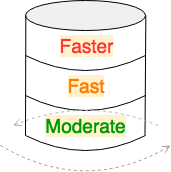
\includegraphics[width=0.15\textwidth]{img/vit_cyl.png}
    \centering
    \caption{schéma rudimentaire\\du projet de test de netteté en mouvement}
    \end{figure}
  Ce qui a été accompli a servi à constituer un document avec des observations et des recommandations qui seront peut-être réutilisés, quand le besoin de tester des caméras se présentera pour l'équipe.
  
  La poursuite du développement de ces protocoles de tests ne semble pas être une priorité pour le moment.
\cleardoublepage
Tout mon stage n'a pas été dédié uniquement à étudier des appareils caméras. J'ai également eu la charge d'établir un benchmark d'algorithmes de suivi fournis avec OpenCV.

\section{Benchmark d'algorithmes avec Open CV}

Durant mon stage, j'ai eu l'opportunité d'utiliser l'API \textbf{OpenCV} pour Python. Cette partie présente d'abord OpenCV, puis la mission qui m'a été confiée de réfléchir à des tests pour comparer des algorithmes de Computer Vision.
  \subsection{Présentation d'Opencv}
  
\begin{minipage}{0.2\textwidth}
  \centering
  
\includegraphics[width=2cm]{img/opencv.png}
\end{minipage}
\hfill%
\begin{minipage}{0.7\textwidth}

  \textit{OpenCV}~\cite{aboutOpenCV} (Open Source Computer Vision Library) est une librairie open source de \textit{Computer Vision} et de \textit{Machine Learning}. Avec une licence BSD, \textit{OpenCV} est simple à utiliser et à modifier pour les business.

\end{minipage}\par
  
La librairie comporte plus de 2500 algorithmes, allant des algorithmes classiques de \textit{Machine Learning} et de \textit{Computer Vision} aux plus modernes. Ces algorithmes permettent notamment de détecter et de reconnaître des objets, tracer les mouvements des objets, ou encore du traitement d'image.

\textit{OpenCV} a des interfaces \textit{C++, Python, Java} ainsi que \textit{MATLAB} et il supporte \textit{Windows, Linux, Android} et \textit{Mac OS}. \textit{OpenCV} continue d'étendre ses compatibilités. Par exemple, une interface pour être utilisé par les processeurs graphiques Nvidia utilisant \textit{ CUDA} est actuellement en cours de développement. La version d'\textit{OpenCV} utilisée durant ce stage est la version \textit{Python} 3.4.1.

  \subsection{Objectif: tests d'algorithmes de tracking}
  
  Cette mission consiste à établir des tests pour comparer différents algorithmes. Ceci passe par la détermination de critères à évaluer et de la mise en place d'une solution pour les évaluer.
  
  \subsubsection{État de l'art}

  \subTrois{Le tracking d'objet}
    
      Le tracking d'objet lui même est la tâche de suivre un ou plusieurs objets dans une scène, de la première apparition à la sortie. Un objet peut être n'importe quel objet qui peut être détecter dans une séquence d'image~\cite{trackingSotA1}. Il peut s'agir d'une voiture qui traverse une intersection. En général, dans un environnement dynamique l'objet et le fond sont susceptibles de changer. La voiture par exemple peut tourner et ainsi changer d'angle de vue et de taille avec la perspective. Le fond avec l'évolution de la luminosité au fil de la journée ou un mouvement de caméra.
  
  En principe la résolution de ces problèmes est complexe. Il est nécessaire de mettre en place une série de contraintes pour qu'il puisse devenir résoluble. Parmi les contraintes qui peuvent aider avec les problématiques de la Computer Vision on compte~:
\begin{itemize}[noitemsep]
  \item Une caméra fixe
  \item Un nombre d'objet connu
  \item La taille des objets connue
  \item Une obstruction des objets limitée
  \item Un déplacement des objets fluide
  \item Pas de changement brutal du fond ou des objets
\end{itemize}
  
    Une fois ces contraintes établies pour générer les vidéos qui serviront de base de travail, des \textit{API} avec leurs lots de solutions existent pour répondre aux besoins en \textit{Computer Vision}. On retiendra principalement celles d'\textbf{Opencv}, tout en s’intéresserant aussi à d'\textbf{autres solutions généralistes}.
    
        Dans la computer Vision, plusieurs types d'algorithmes sont utilisés. Des algorithmes de \textbf{détection}, de \textbf{reconnaissance} et \textbf{tracking}~\cite{Reco}.

    \subTrois{Les solutions fournies par OpenCV}
    \textit{OpenCV} est une librairie qui fournit des API de détection, de reconnaissance et de tracking.
    
        \subQuatre{API de détection}
        OpenCV permet d'utiliser des algorithmes pour détecter un objet sur une image. Un algorithme de détection permet de détecter automatiquement un objet. Cette reconnaissance peut se faire en se focalisant sur les objets en mouvement. Toutefois, cette méthode peut être confrontée à des limitations quand il s'agit d'observer un objet immobile ou obstrué par un objet au premier plan.

Sur OpenCV on retrouve une variété d'algorithmes via son API, dont \textbf{HAAR Cascade}~\cite{HaarOpenCV} qui repose sur du Machine Learning.

Cette méthode peut être utilisée pour suivre un objet image après image, mais risque de le perdre quand il se retrouve à l'arrêt.
      \subQuatre{API de reconnaissance}
        Une fois un objet détecté, il peut être utile de le reconnaître. Dans ce cas, il est nécessaire d'associer les points d’intérêts de l'objet (\textit{features}) à ceux d'une galerie d'objet que l'algorithme a été entraîné à reconnaître.
        
  Les objets que l'on a besoin de reconnaître sont très liés au contexte, les algorithmes de détection sont souvent spécialisés.  Par exemple, depuis Open CV 2.4, une API de reconnaissance de visage est inclue~\cite{FaceReco}.
      \subQuatre{API de tracking}
    Les algorithmes de tracking permettent de suivre un objet. l'algorithme va comparer l'évolution entre plusieurs images successives dans une vidéo. Ces algorithmes permettent de suivre un objet, qu'il se déplace ou non. À la différence d'un algorithme de détection, ils ne permettent pas de repérer automatiquement un objet si on ne le lui pas indiqué initialement. Certains algorithmes sont plus fluides que d'autres, gèrent mieux le changement d'angle de la prise de vue ou de tailles d'un objet, tiennent compte de la perte d'un objet qu'il est supposé suivre.
    
  OpenCV intègre dans sa version 3.4.1 plusieurs fonctions de tracking prête à l'emploi. La plus ancienne \textbf{BOOSTING} a une dizaine d'années alors que les plus récentes comme \textbf{CSRT} ont été ajoutées dans la version la plus récente de l'API.~\cite{APItracking}  
                
  \subTrois{Autres solutions généralistes existantes}
     
       De nombreuses solutions pour le tracking d'objets existent actuellement. Certaines de ces solutions sont apportées par des API de Computer Vision prêtes-à-l'emploi provenant de grands groupes comme \textit{Google}, \textit{Microsoft} et \textit{IBM}~\cite{trackingSotA2}. Cependant ces outils universels ne sont pas toujours utile. Une solution plus spécialisée à un problème donné peut être plus efficace pour sa résolution.
       

\begin{minipage}{0.3265\textwidth}
\begin{figure}[H]
  \centering
  
\includegraphics[width=3cm]{img/tensorflow.png}
    \caption{\\Google Tensorflow}
\end{figure}
\end{minipage}
\begin{minipage}{0.34\textwidth}
\begin{figure}[H]
  \centering
  
\includegraphics[width=3cm]{img/MicrosoftCS.png}
    \label{MS Cognitive Service}
    \caption{MS\\Cognitive Service}
\end{figure}
\end{minipage}
\begin{minipage}{0.3265\textwidth}
\begin{figure}[H]
  \centering
  
\includegraphics[width=3cm]{img/IBM_Watson_Logo_2017.png}
    \caption{\\Watson d'IBM}
\end{figure}
\end{minipage}

Aujourd'hui les algorithmes dans des compétitions de reconnaissance d'objet ne sont toujours pas capable d'avoir des résultats parfaits dans le tracking d'objets multiples~\cite{MOT16}.

  \subsubsection{Contribution sur OpenCV}
     \subTrois{Pertinence et difficulté} Ma mission concerne l'analyse des algorithmes de fonctions de \textbf{suivie} (ou \textbf{tracking}) d'OpenCV.
     
     En effet, les algorithmes concernés serviront à analyser le flux de la circulation routière et piétonne filmé par des caméras de sécurité. Les éléments à tester sont~:
     \begin{itemize}
\item La \textbf{reconnaissance} des objets en premier plan.
\item L’\textbf{identification} des objets en premier plan.
\item Le \textbf{parcours} des objets
\item La \textbf{vitesse d’exécution} en fonction du nombre d’objets et de la résolution de l’image.
\end{itemize}
  
    Les solutions retenues pour chacun de ces points doit tenir en compte des particularités de ce contexte. Parmi ces particularités on peut retenir que l'image est fixe, la qualité risque de varié en fonction de la météo, les zones piétonnes et routières ne varient pas, les objets en mouvement sont des véhicules de tout types et des piétons.
    
    \subTrois{Résolution}
    
    La résolution des difficultés passe par la mise en place matérielle et logicielle du test, et par l'étude des critères à analyser.
    
    \subQuatre{La mise en place}
  Ces tests pour avoir des résultats comparables devront être réalisés sur du matériel avec une configuration connue afin d'éviter les écarts de performance liés au matériel alors que l'on souhaite évaluer les performances du logiciel.
        
  Afin d'avoir des tests reproductibles et que les données attendues soient prévisibles, le flux vidéo qu'analyseront ces algorithmes de \textit{Computer Vision} sera constitué de vidéos enregistrés et correspondant à différentes situations (de circulation ou météorologiques par exemple) pour couvrir au maximum l'efficacité des algorithmes.

    En vue d'établir un benchmark qui répond au mieux aux besoins en l'espèce, deux angles ont été retenus, la précision de l'identification et la vitesse d'exécution.

    \subQuatre{La précision}
    L'algorithme a pour mission d'identifier et de cataloguer les objets filmés et leurs déplacements dans le cadre.

Ces résultats doivent être catalogués dans un log. On attend du log de contenir les objets en mouvement identifiés, les objets reconnus et leurs parcours au travers de différentes zones. Ce log sera analysé et comparé au résultat attendu.

Dans le cadre de la \textbf{reconnaissance} d'un objet en mouvement on peut rencontrer plusieurs cas. Un vrai positif, un objet à détecter a été détecté. Un faux négatif, un objet à détecter n'a pas été détecté. Un faux positif, un objet a été détecté alors qu'il n'y avait pas d'objet à détecter. L'analyse du log doit en tenir compte afin de ne pas favoriser un algorithme trop sensible qui détectera des objets là où rien n'est à analyser.

Pour l'\textbf{identification} d'un objet, soit un objet est correctement identifié soit il ne l'est pas. La situation est la même pour le \textbf{traçage de parcours des objets}. Ce traçage se fait en enregistrant l'entrée et la sortie dans des zones définies pour la caméra (trottoir, passage piété, voie à sens unique...).

L'analyse du log se conclut par l'établissement d'un score qui augmente en fonction des résultats identifiés comme vrai positif  et diminue en fonction des autres.

      \subQuatre{La vitesse d’exécution}
    Les algorithmes n'ont pas nécessairement la même vitesse d'exécution et plus elle est réduite, plus l'algorithme sera apte à analyser un flux continu.
    
    Le test tiendra simplement en compte la durée d'exécution et établira un score en fonction de la durée de la vidéo comme référence.
      \subQuatre{Implémentation}
\textbf{Sélections d'algorithmes de tracking~:}
        
Pour tester différents algorithmes de tracking rapidement,  une fenêtre de sélection de l'algorithme souhaité a été créée. Cette interface est faite en utilisant le module \textbf{tkinter} de \textit{Python}. Dans la liste des algorithmes se trouve pour l'instant les algorithmes inclus dans \textbf{OpenCV}. Ceci évite de modifier manuellement le code à chaque fois que je désire tester un algorithme différent.

% ------------------------------

On va s’intéresser à la partie qui consiste à la sélection d’un algorithme en passant par une interface graphique créée avec tkinker.

\begin{figure}[H]
  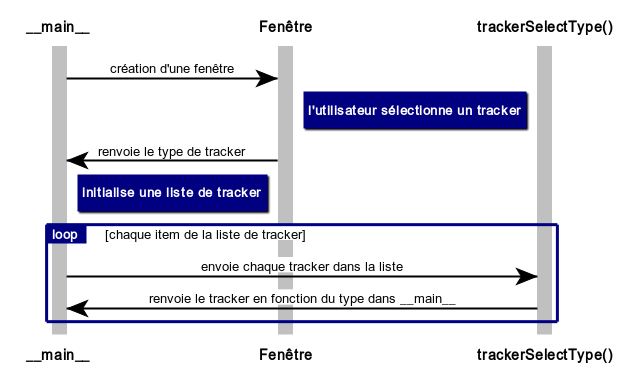
\includegraphics[width=14cm]{img/diag_seq.png}
    \centering
    \caption{Sélection et initialisation\\ de l'algorithme de tracking}
\end{figure}
La première étape est de créer une liste avec le nom de chaque algorithme.

  \begin{minted}[linenos, breaklines, frame=lines, label=Mise en place d'openCV sur Python et de la liste des algorithmes]{python}
import numpy as np
import cv2 as cv
import tkinter as tk
from tkinter.messagebox import showinfo

# Les différents types de trackers inclus dans l'API
    tracker_types = ['BOOSTING', 'MIL', 'KCF', 'TLD', 'MEDIANFLOW', 'GOTURN', 'MOSSE', 'CSRT']
\end{minted}

% ------------------------------
Cette liste va servir à créer une fenêtre avec une liste avec un item à sélectionner

\begin{minted}[linenos, breaklines, frame=lines, label=Fenêtre de sélection de l'algorithme]{python}
fenetre = tk.Tk()
liste = tk.Listbox(fenetre)
for track in tracker_types:
    liste.insert(tracker_types.index(track), track)
liste.pack()
bouton = tk.Button(fenetre,
          text = "Select",
          command = fenetre.quit)
bouton.pack()
fenetre.mainloop()

# Algorithme choisi
tracker_type = tracker_types[liste.curselection()[0]]
\end{minted}
\begin{figure}[H]
  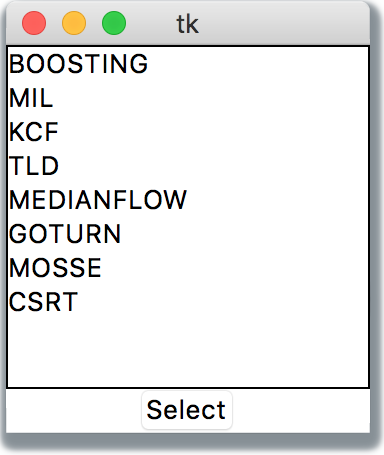
\includegraphics[width=3cm]{img/trackerbox.png}
    \centering
    \caption{boite de dialogue\\pour choisir le tracker}
\end{figure}

% ------------------------------
  On initialise une liste de trackers. Cette liste aura la taille du nombre de \textit{Bounding Box} créées. L'algorithme boosting est sélectionné par défaut afin de créer une liste de trackers, il va être écrasé par un autre tracker.
\begin{minted}[linenos, breaklines, frame=lines, label=Initialisation s'adaptant au nombre de bounding box]{python}
    bbox = [(290, 205, 40, 90),
            (605, 230, 40, 90),
            (700, 250, 40, 90)]
            
for i in range (0,len(bbox)):
        if i == 0:
            trackerselect = [cv.TrackerBoosting_create()]
        else:
            trackerselect.append(cv.TrackerBoosting_create())
    for i in range(0,len(bbox)):
        trackerselect[i] = trackerSelectType(trackerselect[i])
\end{minted}

% ------------------------------

  L'item sélectionné va servir à choisir la fonction pour initialiser un nouveau tracker qui va être inclus dans la liste des trackers. Il écrase le tracker par défaut. Il est nécessaire de repasser par cette fonction à chaque initialisation, autrement la liste de trackers pointera toujours vers le même tracker.

\begin{minted}[linenos, breaklines, frame=lines, label=Attribution de l'algorithme à des trackers]{python}
def trackerSelectType(trackerselect):
    (major_ver, minor_ver, subminor_ver) = (cv.__version__).split('.')
    if int(minor_ver) < 3:
            trackerselect = cv.Tracker_create(tracker_type)
    else:
        if tracker_type == 'BOOSTING':
            trackerselect = cv.TrackerBoosting_create()
        if tracker_type == 'MIL':
...
    return trackerselect
\end{minted}

% ------------------------------

\textbf{La vidéo et les régions d'intérêts des objets à suivre}

Comme on souhaite tester le tracking, les algorithmes sont utilisés dans des situations similaires. Pour cela le programme assure que l'on aura à chaque fois~:
\begin{itemize}[noitemsep]
\item La même vidéo.
\item Les mêmes zones d’intérêt sélectionnées. 
\end{itemize}
De légères différences dans la zone sélectionnée pour encadrer l'objet à suivre peuvent changer sensiblement le comportement de l'algorithme. Idéalement cette zone doit contenir au maximum l'objet avec un minimum d'arrière plan. Ceci peut être compliqué quand on analyse des formes non rectangulaires comme un cycliste sur son vélo.

Plusieurs vidéos ont été sélectionnées pour ce test. Une première, \textit{Shibuya} a été choisie car elle permet de voir la différence de comportement sur des objets de différentes tailles (voiture, bus, et arrière d'une voiture) et des obstacles (vue obstruée par le feu tricolore, la foule de piéton).

Les régions d'intérêts sont entrées dans un \textbf{tableau de tuples} (collection ordonnée d'attributs relatifs à un même objet) qui contiennent les coordonnées de chaque \textit{bounding box} (sélection rectangulaire de l'objet à suivre). L'utilisation de la bounding box se fait sous forme de boucle dont l'index s'adapte à la taille de se tableau de tuples. Ainsi en ajoutant ou retirant simplement un tuple dans ce tableau, le programme va pouvoir les suivre sans autre modification.

On peut déjà s'apercevoir en observant la vidéo que le comportement de ces \textit{Bounding Box} varie en fonction des algorithmes.

\begin{figure}[H]
  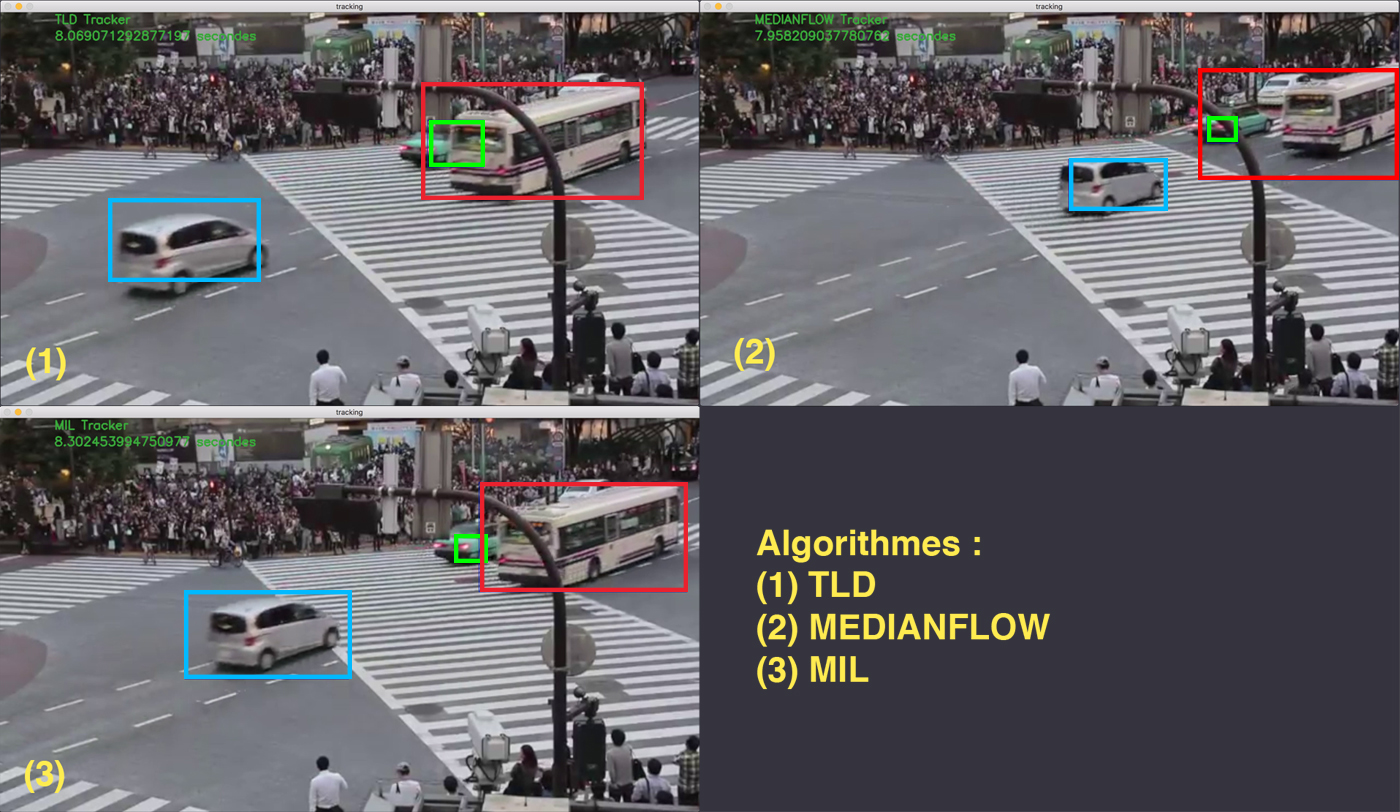
\includegraphics[width=0.7\textwidth]{img/algodiff.jpg}
    \centering
    \caption{Différence de résultats entre différents algorithmes à environ 8 secondes d'exécution.}
\end{figure}

Ces \textit{Bounding Box} vont avoir des temps d’exécutions plus ou moins long et vont parfois échouer à suivre chaque voiture sur la totalité de leur trajet. Avec ces informations, on peut commencer à l'élaborer un score pour chaque algorithme. L'incapacité à suivre des objets se déplaçant en ligne droite est éliminatoire et est indexé sur le temps d’exécution.

\begin{table}[H]
  \centering
  \label{my-label}
\begin{tabular}{|l|l|l|l|}
\hline
\rowcolor[HTML]{FFFFC7} 
Algorithme & Temps (secondes)   & Perte & \begin{tabular}[c]{@{}l@{}}Score\\ \tiny{\((3-Pertes) * (100/3)\)}\\\tiny{\( * ( Temps * Dur\acute{e}e)\)}\end{tabular}\\ \hline
Boosting   & 51.208574295043945 & 2     & 3,254663286                                                                     \\ \hline
MIL        & 54.95484709739685  & 2     & 3,032792838                                                                     \\ \hline
KCF        & 35.16063404083252  & 2     & 4,740149636                                                                     \\ \hline
TLD        & 110.28673601150513 & 3     & 0                                                                               \\ \hline
\textbf{MEDIANFLOW} & \textbf{24.363162994384766} & \textbf{0} & \textbf{20,5227868}                                                             \\ \hline
\end{tabular}
  \caption{Exemple de score pour différents algorithmes sur \textit{Shibuya}}
\end{table}

On peut alors observer sur cinq algorithmes un écart très important dans les temps d’exécution et la capacité à suivre un objet.

La vidéo \textit{Shibuya} a comme inconvénient un encodage qui conduit à une exécution très lente des algorithmes. La vidéo de \textbf{4,6 secondes} peut avoir un temps d’exécution de  l'algorithme TLD proche de \textbf{2 minutes}. Si cela peut être pénible lorsque l'on souhaite effectuer plusieurs tests successifs, ceci permet toutefois de mettre en exergue les différences de performances.

Lors de la suite de l'élaboration des tests, d'autres vidéos ont été privilégiées.

\textbf{Zones d'entrées et de sorties}

Un autre vidéo présente dans une intersection prise en coopération avec la ville cliente a servi pour les tests. Avec cette vidéo les temps d’exécution des algorithmes était bien plus proche de la durée de la vidéo.

Pour utiliser ces zones il a fallu choisir le critère pour déterminer quand un objet est ou non dans une zone. Pour cela les coordonnées Bounding Box sont exploitées. Plutôt que de considérer un objet comme dans une zone quand elle se superpose à la \textit{Bounding Box}, l'objet est considéré dans la zone quand son centre est dans la zone. 

Une fois ce critère choisi il a été possible d'afficher le parcours qu'effectue la \textit{Bounding Box} pour simplifier l'observation humaine. Dans ce même soucis d’observation, un message est affiché quand un objet est dans une zone. 

\begin{figure}[H]
  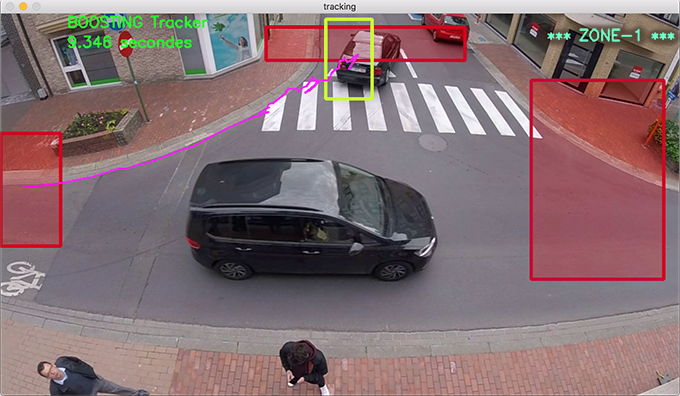
\includegraphics[width=0.6\textwidth]{img/ALGOZONE.png}
    \centering
    \caption{Objet entrant dans une zone}
\end{figure}

Il arrive que l'objet n'arrive pas à entièrement entrer dans la zone mais se superpose, choisir l'ensemble de la surface de la \textbf{Bounding Box} est plus favorable à produire des \textbf{faux positifs}.

\begin{figure}[H]
  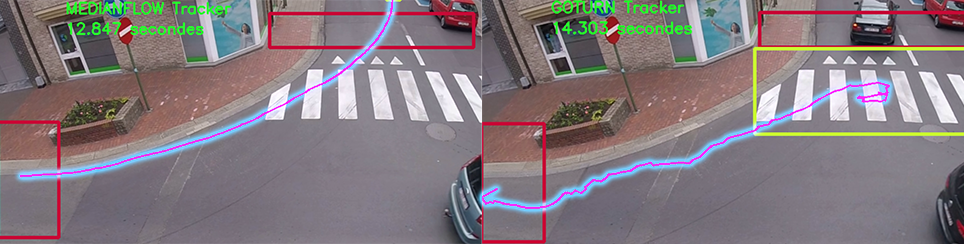
\includegraphics[width=0.9\textwidth]{img/path.png}
    \centering
    \caption{Différence de trajet entre deux algorithmes en magenta surligné}
\end{figure}

Dans le cas de figure de l'algorithme \textbf{Goturn}, l'objet était partiellement superposé dans la zone centrale. Choisir un paramètre plus restreint comme le centre a permis d'éviter un \textbf{faux positif}. 

\textbf{Création d'un log}

 Pour la création du log j'ai utilisé la librairie Python \textbf{logging}~\cite{log}. Cette librairie permet de simplement créer un fichier de log en fonction de l'activité du programme. Ce fichier a vocation à garder une trace de la dite activité et ainsi être utilisé pour comparer des résultats. Il enregistre quel algorithme est utilisé lors de la session, la position toute les trente frames, et quand l'objet entre et sort d'une zone.

\textbf{Élaboration d'un benchmark}

 % -------------------------`
 % -------------------------
 % |   |   |   |   |   |   |
 % -------------------------
  Pour affiner le benchmark par rapport au tableau de score précédent, des critères ont été ajoutés. Ces critères sont surtout qualitatifs et sont alors difficilement quantifiables. Avec la constatation des différences de performances entre les algorithmes, j'ai passé la vitesse d’exécution comme une variable qualitative. Au vu de la variabilité d'un critère comme les pertes en fonction de la vidéo, j'ai préféré en faire une variable qualitative en fonction de la capacité à ne pas perdre et sous le nom de «~\textit{Précision}~». 
% Please add the following required packages to your document preamble:
% \usepackage[table,xcdraw]{xcolor}
% If you use beamer only pass "xcolor=table" option, i.e. \documentclass[xcolor=table]{beamer}
\begin{table}[H]
\centering
\begin{tabular}{|c|c|c|c|c|c|}
\hline
\rowcolor[HTML]{3166FF} 
{\color[HTML]{FFFFFF} \textbf{Nom}}          & {\color[HTML]{FFFFFF} \textbf{Vitesse}}                         & {\color[HTML]{FFFFFF} \textbf{Adapte taille}}               & {\color[HTML]{FFFFFF} \textbf{\begin{tabular}[c]{@{}c@{}}repère\\ quand perdu\end{tabular}}} & {\color[HTML]{FFFFFF} \textbf{Fluidité}} & {\color[HTML]{FFFFFF} \textbf{Précision}} \\ \hline
\rowcolor[HTML]{F8A102} 
\cellcolor[HTML]{DAE8FC}\textbf{Boosting}    & {\color[HTML]{333333} \textbf{lent --}}                         & \cellcolor[HTML]{FE0000}{\color[HTML]{FFFFFF} \textbf{non}} & \cellcolor[HTML]{FE0000}{\color[HTML]{FFFFFF} \textbf{non}}                                  & \textbf{--}                              & \textbf{--}                               \\ \hline
\rowcolor[HTML]{FFFE65} 
\cellcolor[HTML]{DAE8FC}\textbf{MIL}         & {\color[HTML]{333333} \textbf{len -}}                           & \cellcolor[HTML]{FE0000}{\color[HTML]{FFFFFF} \textbf{non}} & \cellcolor[HTML]{FE0000}{\color[HTML]{FFFFFF} \textbf{non}}                                  & \textbf{-}                               & \textbf{-}                                \\ \hline
\cellcolor[HTML]{DAE8FC}\textbf{KCF}         & \cellcolor[HTML]{FFFE65}\textbf{lent -}                         & \cellcolor[HTML]{FE0000}{\color[HTML]{FFFFFF} \textbf{non}} & \cellcolor[HTML]{32CB00}\textbf{oui}                                                         & \cellcolor[HTML]{32CB00}\textbf{+}       & \cellcolor[HTML]{FFFE65}\textbf{-}        \\ \hline
\rowcolor[HTML]{FE0000} 
\cellcolor[HTML]{DAE8FC}\textbf{TLD}         & {\color[HTML]{FFFFFF} \textbf{lent ---}}                        & \cellcolor[HTML]{32CB00}\textbf{oui}                        & {\color[HTML]{FFFFFF} \textbf{non}}                                                          & {\color[HTML]{FFFFFF} \textbf{---}}      & {\color[HTML]{FFFFFF} \textbf{---}}       \\ \hline
\rowcolor[HTML]{32CB00} 
\cellcolor[HTML]{DAE8FC}\textbf{Median Flow} & \cellcolor[HTML]{FFFE65}\textbf{lent -}                         & \textbf{oui}                                                & \textbf{oui}                                                                                 & \textbf{+}                               & \textbf{+}                                \\ \hline
\cellcolor[HTML]{DAE8FC}\textbf{Goturn}      & \cellcolor[HTML]{F8A102}{\color[HTML]{333333} \textbf{lent --}} & \cellcolor[HTML]{32CB00}\textbf{oui}                        & \cellcolor[HTML]{FE0000}{\color[HTML]{FFFFFF} \textbf{non}}                                  & \cellcolor[HTML]{FFFE65}\textbf{-}       & \cellcolor[HTML]{F8A102}\textbf{--}       \\ \hline
\rowcolor[HTML]{32CB00} 
\cellcolor[HTML]{DAE8FC}\textbf{MOSSE}       & \cellcolor[HTML]{FFFE65}\textbf{lent -}                         & \cellcolor[HTML]{FE0000}{\color[HTML]{FFFFFF} \textbf{non}} & \textbf{oui}                                                                                 & \textbf{+}                               & \textbf{+}                                \\ \hline
\cellcolor[HTML]{DAE8FC}\textbf{CSRT}        & \cellcolor[HTML]{F8A102}\textbf{lent --}                        & \cellcolor[HTML]{32CB00}{\color[HTML]{333333} \textbf{oui}} & \cellcolor[HTML]{FE0000}{\color[HTML]{FFFFFF} \textbf{non}}                                  & \cellcolor[HTML]{32CB00}\textbf{+}       & \cellcolor[HTML]{FFFE65}\textbf{-}        \\ \hline
\end{tabular}
\caption{benchmark de différents algorithmes de tracking}
\end{table}



Un score n'est plus déduit, mais les différences restent facilement visibles.


  \subsection{Résultats et améliorations possibles}
    En l'état, le programme connaît encore plusieurs lacunes. 
    
    Il est fait pour lancer les algorithmes fournis par OpenCV. Cece le rend \textbf{limité par ces algorithmes implémentés de base}. Les algorithmes développés à part ne seront pas compatibles et demanderont des refontes importantes du programme pour y être utilisable. 
    
    Configurer le programme peut s'avérer \textbf{laborieux}. Sélectionner les zones d’intérêt se fait en rentrant des \textbf{coordonnées} d’abscisse, d'ordonnée, de longueur et de la largeur à la main.
Pour entrer un \textbf{temps} à laquelle une voiture est attendu dans une zone, il faut choisir une frame. Le temps en utilisant une horloge ne fonctionne pas car les algorithmes ont des temps d'exécutions différents. Trouver ces informations demande de procéder par tâtonnements et peut demander un nombre important d'essais.
    
    Également le programme n'est doté que d'une \textbf{faible automatisation}. Il n'est pas possible avec de programme d'automatiser avec certitude quand un objet entre ou sort d'une zone, car aucun de ces algorithmes de tracking n'est parfaitement fiable. 

  Parmi les objectifs posés lors de la réflexion autour des tests d'algorithmes de tracking se trouvaient les notions de \textbf{faux et vrais positifs}. Lors de la conception du programme je me suis retrouvé confronté à des problèmes pour reconnaître un faux positif. Par exemple, certains algorithmes ne sont pas capables de comprendre quand l'objet est perdu. Certains algorithmes peuvent voir leur zone d'analyse faire des «~sauts~» quand ils perdent l'objet et se retrouver dans la zone attendue. De même algorithme peut se mettre à suivre un mauvais objet quand il en croise un autre. 

 Effectuer un \textbf{benchmark} des algorithmes n'est pas parfaitement rigoureux. Les différences de vitesses changent en fonction de l'encodage de la vidéo. La capacité d'un algorithme à suivre un objet dépend grandement de la zone d’intérêt sélectionnée au départ. Il est possible qu'une zone d’intérêt favorise plus un algorithme qu'un autre.
 
 L'observation humaine reste essentielle dans ces tests.
\cleardoublepage
\section{Bilan des acquis}

  Ces trois premiers mois de stages ont été l'occasion de travailler dans un environnement de travail qui laisse une grande place à l'\textbf{autonomie}. 

  Ce stage a d'abord été l'occasion d'appliquer mes connaissances acquises en MIAGE, tel que des \textbf{notions de réseaux} à la connexion de caméra IP, ou à m'abstraire pour résoudre des problèmes et concevoir des solutions. 

  Pour les besoins du stage j'ai appris le langage de programmation \textbf{Python}. J'ai notamment pu explorer comment fonctionne les rudiments de la syntaxe Python et l'utilisation de librairies comme \textit{tkinter} pour créer une interface graphique sommaire ou \textit{logger} pour des logs.

  Ceci a été fait dans le cadre de mission liée à la \textbf{Computer Vision}, domaine que j'ai pu découvrir à cette occasion, et mis en application avec \textbf{OpenCV}.

\newpage

\nocite{*}
\printbibliography

\end{document}
